\subsection{Reasons of an Overhaul}
\paragraph{}
The original architecture of the vehicle was already a good basis for the
realisation of a line tracking car. However, manual manoeuvring tests by
remote control have revealed some driving faults. Misconduct that could
be embarrassing in an autonomous driving mission. Given that our robot
will certainly not be as adaptive as a human in its driving, it is
interesting to ease the maneuvers and correct some mobility deficiencies.

\subsubsection{Problems identified and changes to be expected}
\paragraph{}
Some of the shortcomings noted are listed as follows:
\begin{itemize}
    \item Loss of control due to high front wheel slippage during high speed turns.
    \item In case of sharp turn, locking of the inner wheel on the bend caused by
    the central component box.
    \item Lack of firmness of the front wheel guiding created by a large backlash.
    \item Uncontrolled spinning of the rear wheels when acceleration from a
    standstill or deceleration from high speeds.
\end{itemize}
And some others component have to be implemented to the initial structure in order
to be an optimal support for autonomous driving such as:
\begin{itemize}
    \item The installation of a camera to see and locate the line to follow.
    \item Hosting a Raspberry Pi card to manage the control computations.
    \item Keep space for the rest of the essential components such as the battery,
    ESC, cables, etc.
\end{itemize}

\subsection{Front Wheel Steering}

\subsubsection{Front wheel slip}
\paragraph{}
One of the major problems that needs to be corrected, a problem that could impact
autonomous driving, is the significant slipping of the front wheels when the steering
angle is too large  at high speed.

\paragraph{}
To correct this defect, the best solution would be to improve road handling by
increasing the car's grip. To do this, the wheels would have to be changed from
smooth tires to studded wheels.
However, considering the stock of parts available at ENSTA Bretagne, unless you
make an order which would take some time, we did not have better wheels than the
ones proposed.

\subsubsection{Ackermann steering geometry}
\paragraph{}
Nevertheless, we have come up with another solution inspired by normal cars.
The principle of this solution comes from the geometry, especially the steering
geometry of Ackermann.

\paragraph{}
The intention is to avoid the need for tyres to slip sideways when following the
path around a curve. The geometrical solution to this is for all wheels to have
their axles arranged as radii of circles with a common centre point.  As the rear
wheels are fixed, this centre point must be on a line extended from the rear axle.
Intersecting the axes of the front wheels on this line as well requires that the
inside front wheel be turned, when steering, through a greater angle than the
outside wheel.

\begin{figure}[!ht]
    \begin{center}
        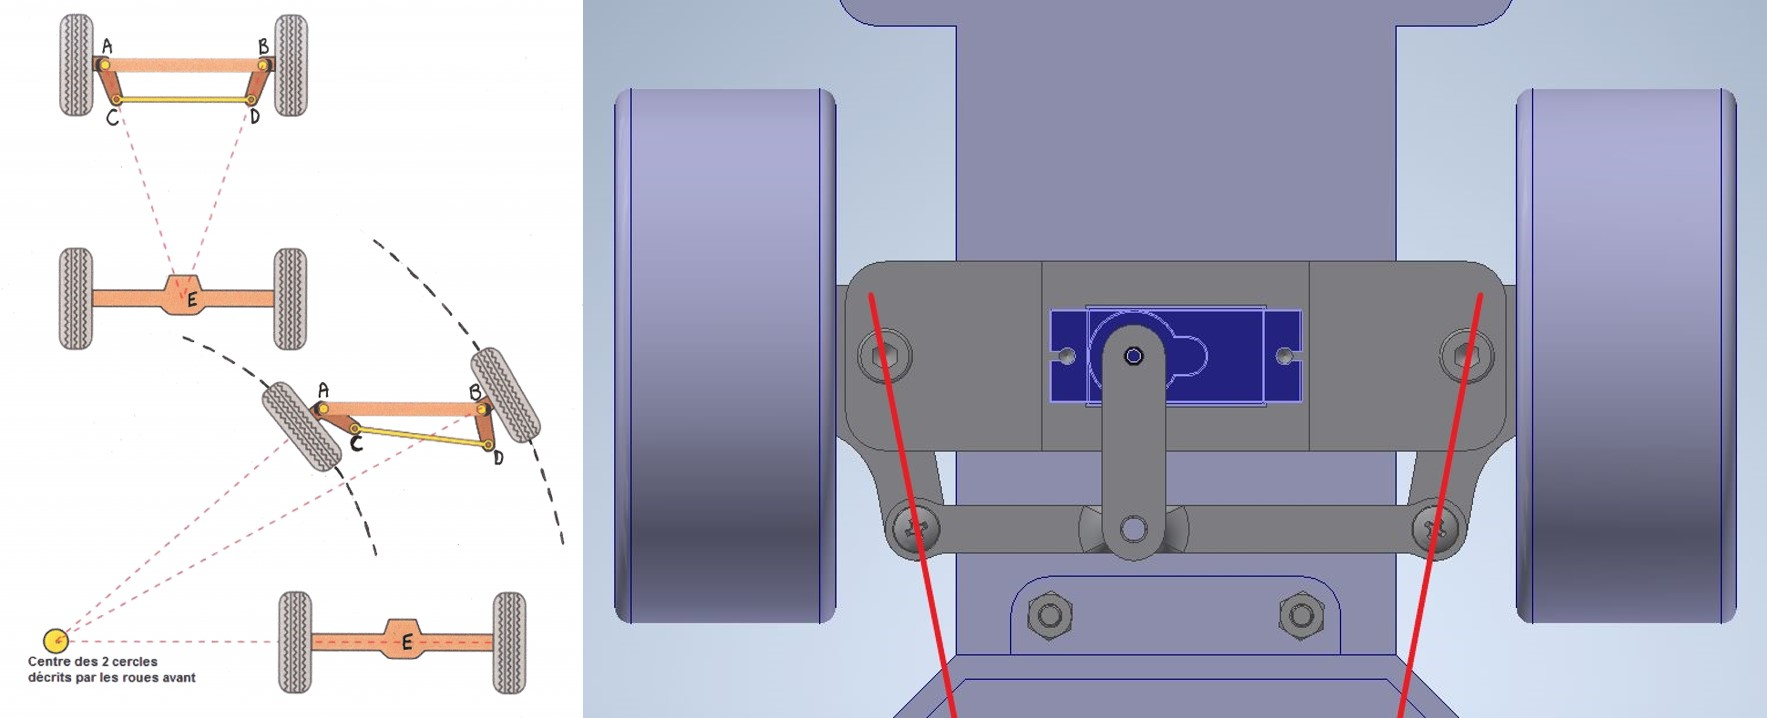
\includegraphics[scale=0.45]{Images/steering.jpg}
    \end{center}
    \caption{Steering system}
    \label{fig:raspi_config}
\end{figure}

A simple approximation to perfect Ackermann steering geometry may be generated by
moving the steering pivot points inward so as to lie on a line drawn between the
steering kingpins and the centre of the rear axle.

\paragraph{}
We have therefore redesigned the pivot points to respect this geometry. We also
took advantage of this to improve the bearing embedding system that connects the
bearing to the wheel so that the steering wheels are held more firmly.

\subsection{Front Camera Support}

\subsubsection{Camera support structure}
\paragraph{}
We then had to implement the camera that would allow our robot car to have eyes
on the road.

In order to position it correctly, the camera had to be able to stand back enough
on the road in front of it and the angle of view had to be horizontal enough to see
far away but with a high enough incidence to identify the line without being
hindered by the sun's reflections.

\begin{figure}[!ht]
    \begin{center}
        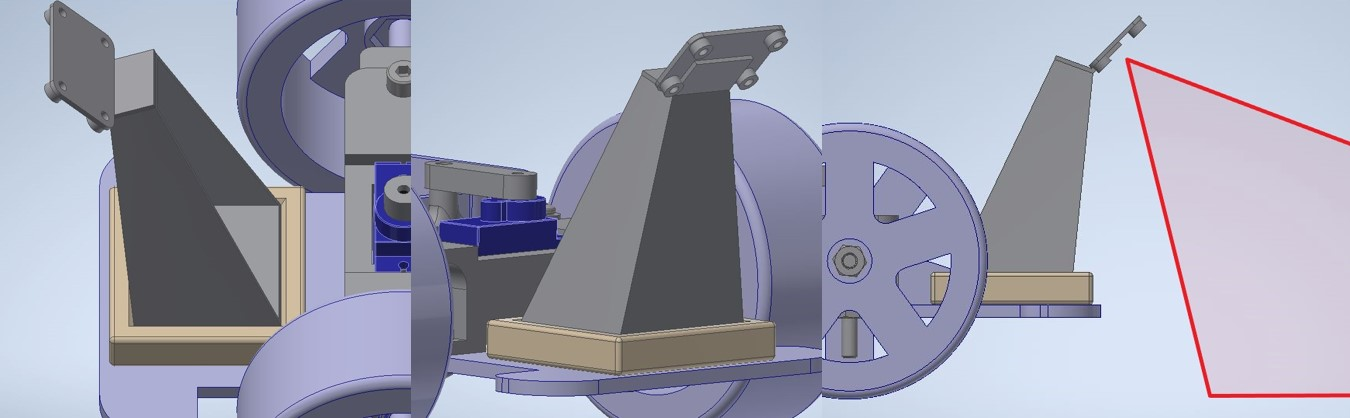
\includegraphics[scale=0.58]{Images/camera_support.jpg}
    \end{center}
    \caption{Front camera support structure}
    \label{fig:raspi_config}
\end{figure}

We have therefore designed a structure that raises the camera a few centimetres
above the chassis and tilts it at 45 degrees towards the ground. 

\subsubsection{Annoying vibrations}
\paragraph{}
Our car will be driven in a natural environment and the ground will probably
not be totally smooth but slightly bumpy and gravelly. The chassis will be
subjected to many vibrations and at the same time, the camera to which it is
connected will also be subjected to them, which can be quite annoying
afterwards in the image processing.

\paragraph{}
We therefore had to find a solution to try to reduce these disturbances.
One of the simple mechanical solutions is to dampen the vibrations in the
connection between the chassis and the camera by using for example a silentblock.
As a silentblock, a soft synthetic foam seems to be a good choice to counteract
these vibrations. (See Figure 5 for more details)

\subsection{Component Hosting Box}

\subsubsection{Additional space}
\paragraph{}
In order to host the necessary additional electronics we needed to increase the
space to host the components. We redesigned the box by increasing its width.
In its new dimensions, the box offers twice as much space without unbalancing
the overall structure.

\begin{figure}[!ht]
    \begin{center}
        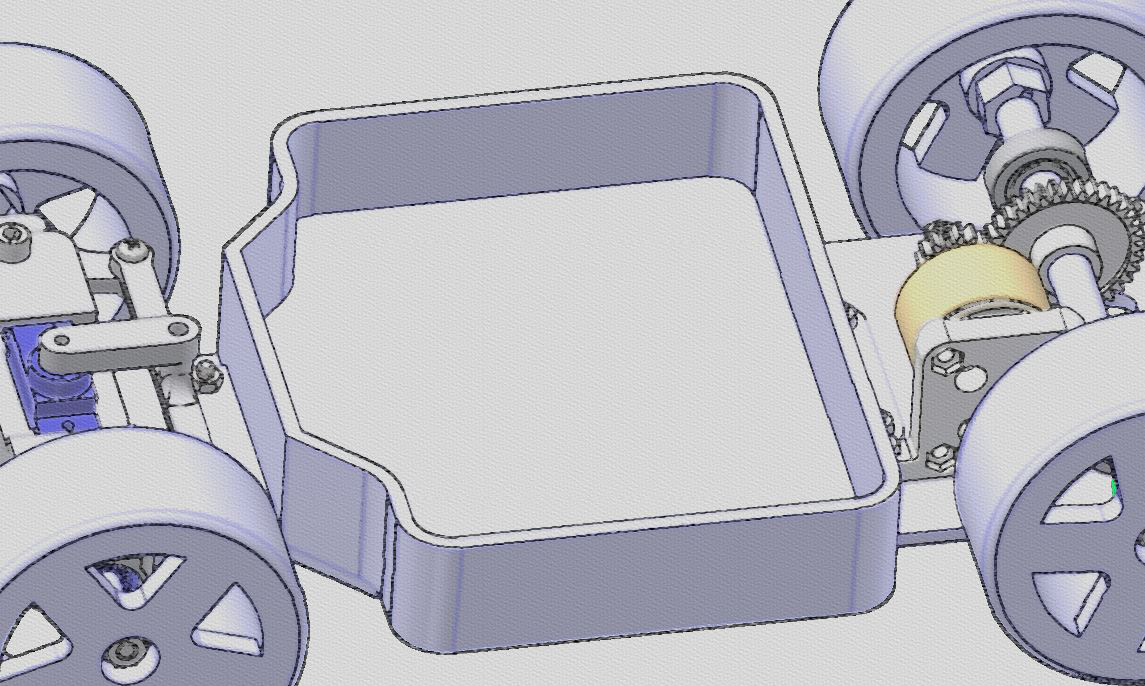
\includegraphics[scale=0.45]{Images/kart_central_box.png}
    \end{center}
    \caption{Central component box}
    \label{fig:raspi_config}
\end{figure}

\subsubsection{Carved box}
\paragraph{}

In the process of creating a new box, we took the opportunity to correct one
of the problems caused by the front corners that blocked the steering wheels
when they were fully steered. So we took the care to add two notches in
the place of these corners to allow the wheels to move without hitting them.
(See Figure 6 for more details)

\subsection{Expectations and Reality}
\paragraph{}
As you may probably know, there is a difference between expectations and the
actual reality.

\paragraph{}
The plans were good, but an unprecedented event came to modify them, as a
consequence of the proliferation of covid-2019, the school had to close its
doors. Deprived of manufacturing means and having only one prototype for the
group, we had to stick to what was already done. With DIY, hot glue and a
bit of common sense we were able to come up with a modest but acceptable
structure.

\paragraph{}
In the final model, the proposed solutions include Ackermann's steering
system and the system for embedding the bearings connected to the steering
wheels. The front camera support had to be totally modified but the intentions
are the same even though there is no damping system. And the housing box has
remained the same but has been doubled on a second floor to contain the
electronic components.
By limiting the rotational movement of the steering wheels, we can ensure
that the front wheels do not get stuck. (See Figure 7 for more details)

\paragraph{}
Although the final structure of our car does not have all the improvement
imagined, it still in acceptable condition for autonomous driving in an
environment like a traditional athletics track.

\begin{figure}[!ht]
    \begin{center}
        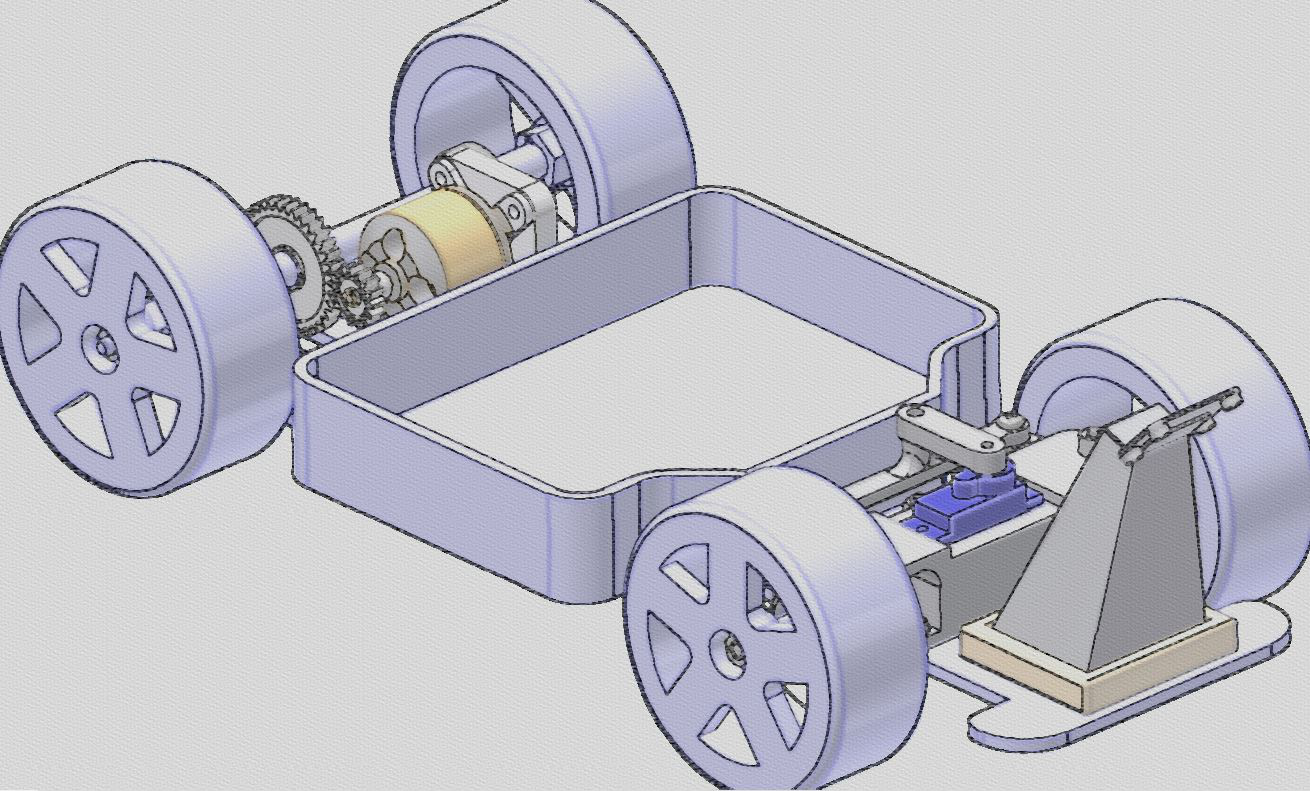
\includegraphics[scale=0.4]{Images/plan_global.png}
        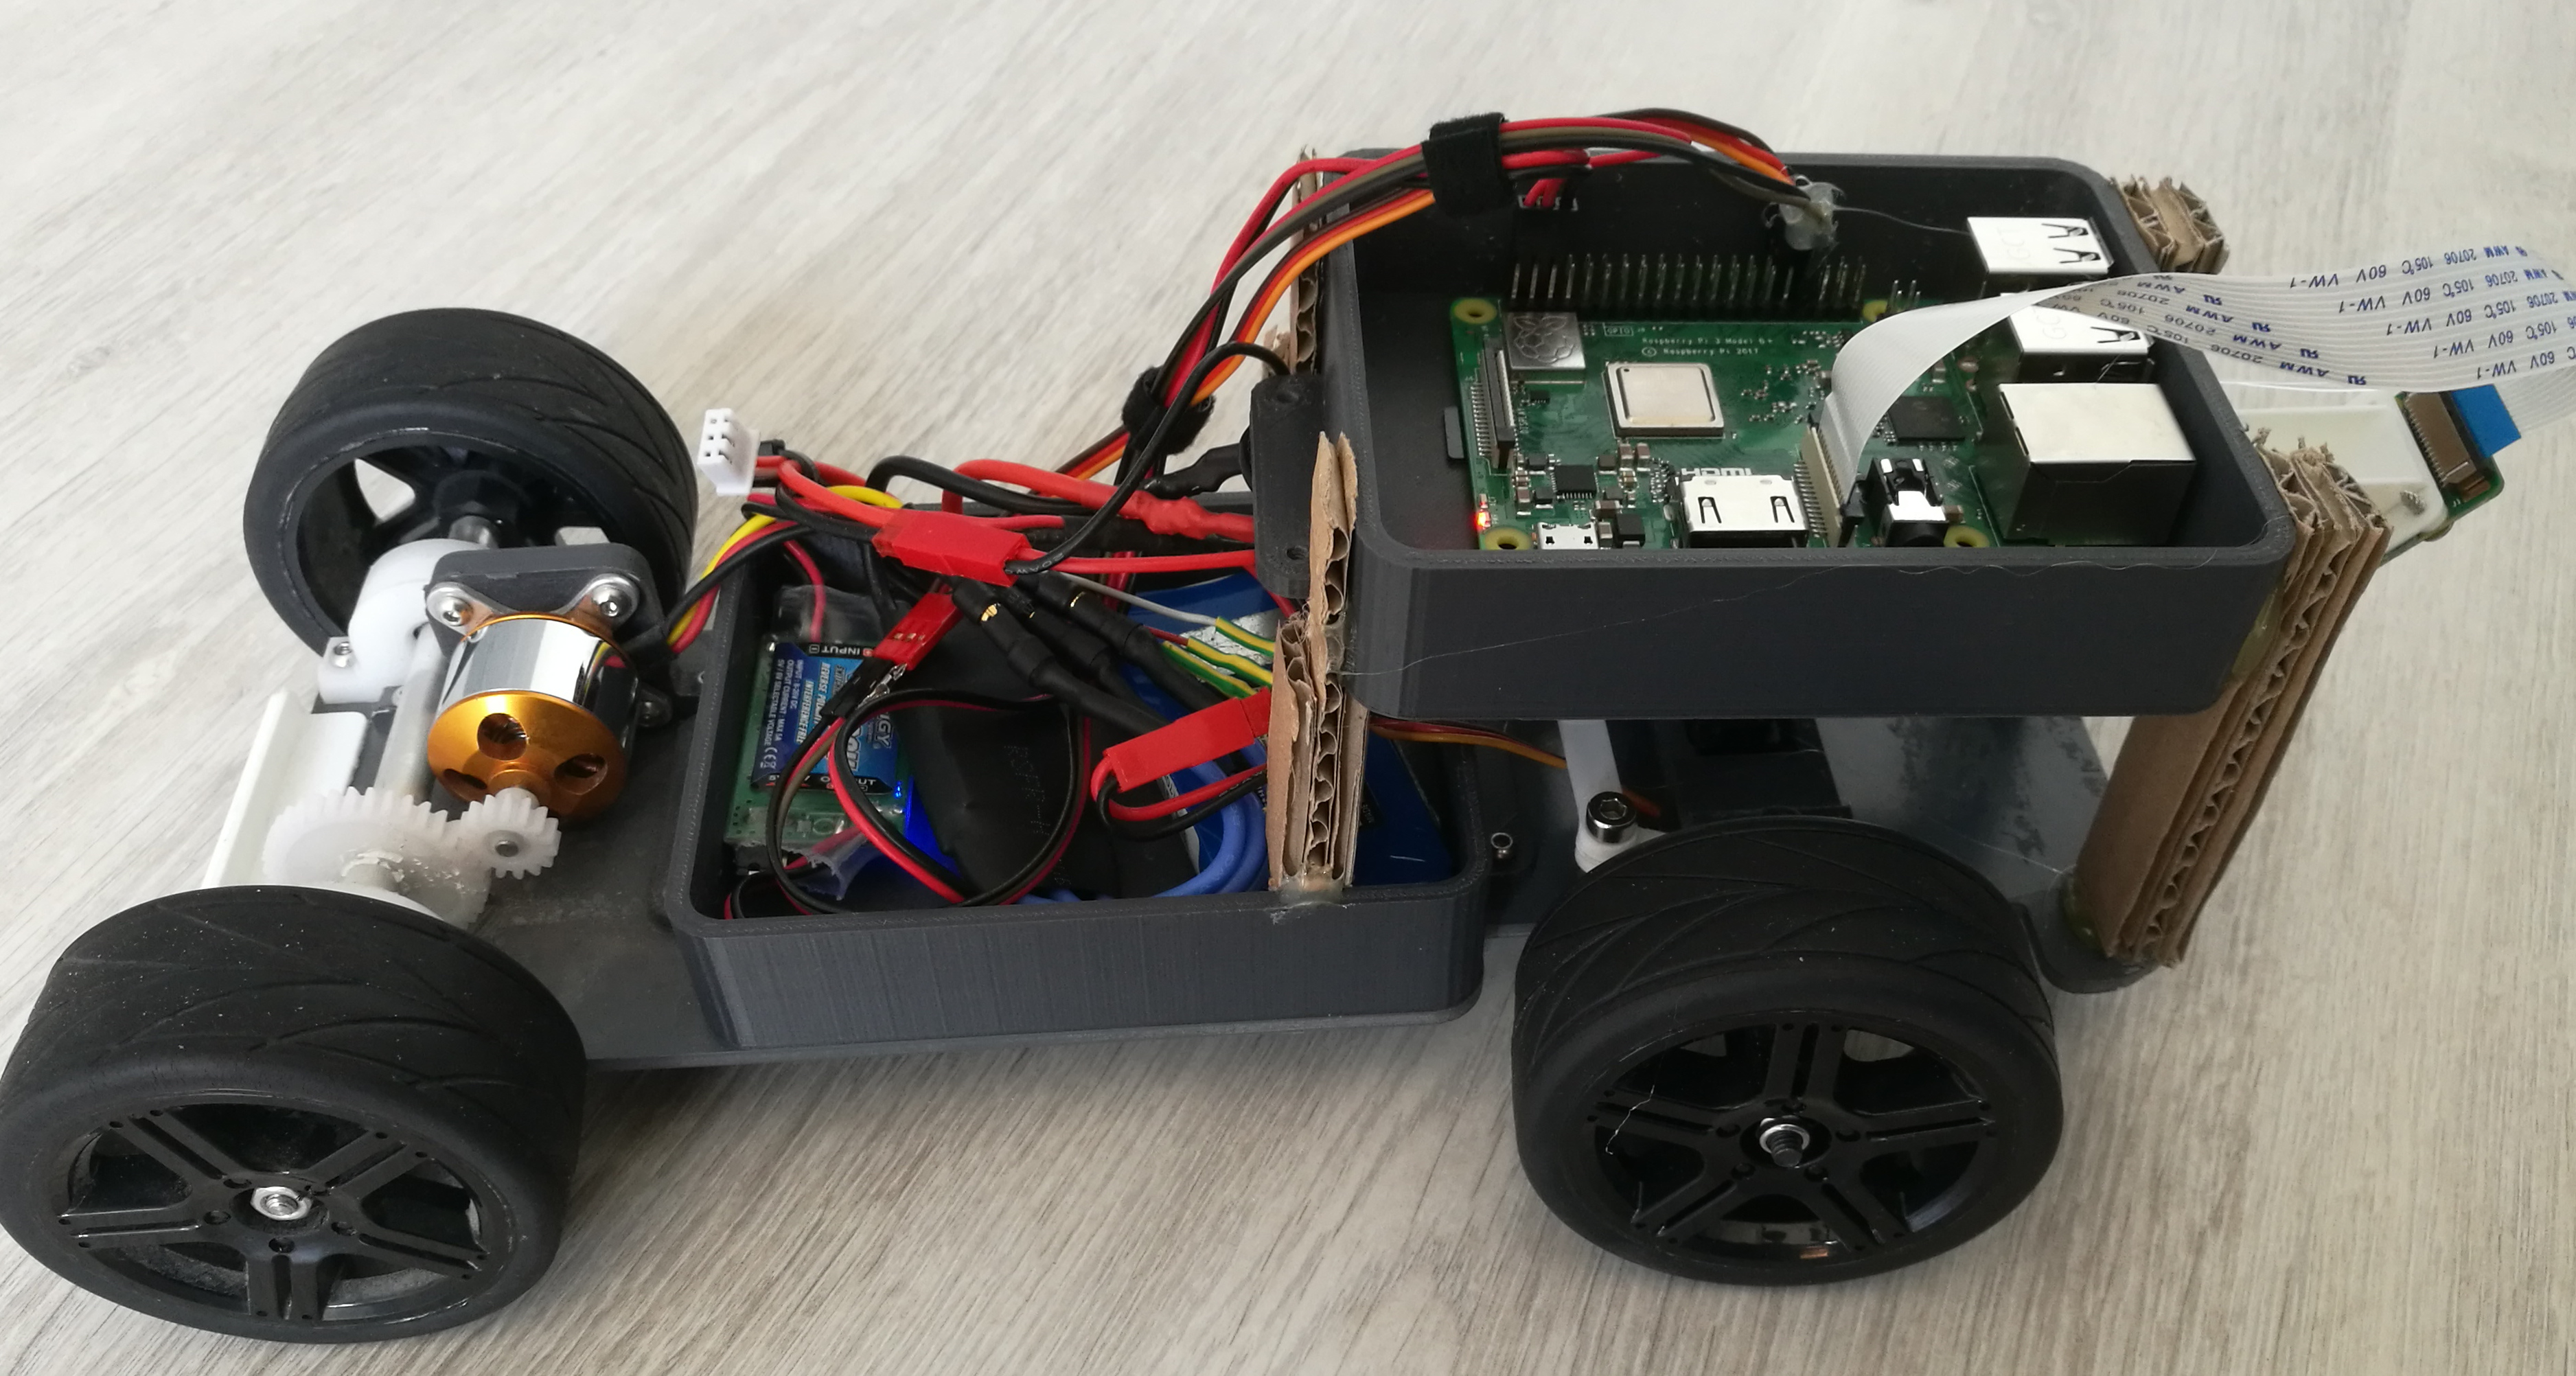
\includegraphics[scale=0.135]{Images/Kart_overview_1.jpg}
    \end{center}
    \caption{Expextations and reality}
    \label{fig:raspi_config}
\end{figure}